In an Isosceles triangle the angles opposite to sides of equal length are equal.Therefore the angles $\angle ABC=\angle ACB$ and $\angle DBC=\angle DCB$.Let the vertex $B$ be at origin and not lose generality.Since the two triangles are isosceles,$\norm{\vec{B}-\vec{D}}=\norm{\vec{C}-\vec{D}}$ and $\norm{\vec{A}-\vec{B}}=\norm{\vec{A}-\vec{C}}$.
The triangles $\triangle ABC$ and $\triangle DBC$ are isosceles triangles,so
\begin{align}
    \norm{\vec{A}-\vec{B}} = \norm{\vec{A}-\vec{C}}\label{eq:solutions/1/32/eq:1}\\
    \norm{\vec{D}-\vec{B}} = \norm{\vec{D}-\vec{C}}\label{eq:solutions/1/32/eq:2}
\end{align}
From equation \eqref{eq:solutions/1/32/eq:1},we get
\begin{multline}
    {\brak{\vec{A}-\vec{B}}^T\brak{\vec{A}-\vec{B}}}={\brak{\vec{A}-\vec{C}}^T\brak{\vec{A}-\vec{C}}}\\
    {\brak{\vec{A}-\vec{B}}^T\brak{\vec{A}-\vec{D}+\vec{D}-\vec{B}}}=\\{\brak{\vec{A}-\vec{C}}^T\brak{\vec{A}-\vec{D}+\vec{D}-\vec{C}}}\\
    {\brak{\vec{A}-\vec{B}}^T\brak{\vec{D}-\vec{B}}}=\\
    {\brak{\vec{A}-\vec{C}}^T\brak{\vec{D}-\vec{C}}
    +\brak{\vec{B}-\vec{C}}^T\brak{\vec{A}-\vec{D}}}\label{eq:solutions/1/32/eq:3}
\end{multline}
Doing the below calculation,we get
\begin{multline}
    {\brak{\vec{C}-\vec{B}}^T\brak{\vec{A}-\vec{B}}-\brak{\vec{C}-\vec{B}}^T\brak{\vec{D}-\vec{B}}}=\\
    {\brak{\vec{A}-\vec{C}}^T\brak{\vec{B}-\vec{C}}-\brak{\vec{D}-\vec{C}}^T\brak{\vec{B}-\vec{C}}}\\
    {\brak{\vec{C}-\vec{B}}^T\brak{\vec{A}-\vec{D}}}={\brak{\vec{A}-\vec{D}}^T\brak{\vec{B}-\vec{C}}}\label{eq:solutions/1/32/eq:6}
\end{multline}
\begin{figure}[!h]
    \centering
    \resizebox{\columnwidth}{!}{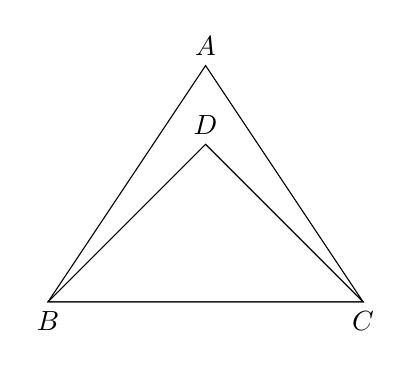
\begin{tikzpicture}
    \coordinate (B) at (0,0);
    \coordinate (A) at (2,3);
    \coordinate (C) at (4,0);
    \coordinate (D) at (2,2);
    \draw (A)node[above]{$A$}--(B)node[below]{$B$}--(C)node[below]{$C$}--cycle;
    \draw (D)node[above]{$D$}--(B)node[]{}--(C)node[]{}--cycle;
\end{tikzpicture}
}
    \caption{Isosceles triangles with common base BC}
    \label{eq:solutions/1/32/myfig:1}
\end{figure}
Since $\brak{\vec{A}-\vec{D}}^T\brak{\vec{B}-\vec{C}}$=${\brak{\vec{B}-\vec{C}}^T\brak{\vec{A}-\vec{D}}}$, the equation \eqref{eq:solutions/1/32/eq:6} can be written as
\begin{align}
    {\brak{\vec{B}-\vec{C}}^T\brak{\vec{A}-\vec{D}}}&={\brak{\vec{C}-\vec{B}}^T\brak{\vec{A}-\vec{D}}}\\
    {\brak{\vec{B}-\vec{C}}^T\brak{\vec{A}-\vec{D}}}&=-{\brak{\vec{B}-\vec{C}}^T\brak{\vec{A}-\vec{D}}}\\
    2{\brak{\vec{B}-\vec{C}}^T\brak{\vec{A}-\vec{D}}}&=0\\
    \brak{\vec{B}-\vec{C}}^T\brak{\vec{A}-\vec{D}}&=0\label{eq:solutions/1/32/eq:7}
\end{align}
Taking the inner product of $A-B,B-D$ and $A-C,D-C$,we get
\begin{align}
    \cos\angle ABD=\frac{\brak{\vec{A}-\vec{B}}^T\brak{\vec{D}-\vec{B}}}{\norm{\vec{A}-\vec{B}}\norm{\vec{D}-\vec{B}}}\\
    \cos\angle ACD=\frac{\brak{\vec{A}-\vec{C}}^T\brak{\vec{D}-\vec{C}}}{\norm{\vec{A}-\vec{C}}\norm{\vec{D}-\vec{C}}}
\end{align}
Subtracting the above equations we get 
\begin{align}
    \cos\angle ABD-\cos\angle ACD\\
    =\frac{\brak{\vec{A}-\vec{B}}^T\brak{\vec{D}-\vec{B}}-\brak{\vec{A}-\vec{C}}^T\brak{\vec{D}-\vec{C}}}{\norm{\vec{A}-\vec{C}}\norm{\vec{D}-\vec{C}}}\\
    =\frac{\brak{\vec{B}-\vec{C}}^T\brak{\vec{A}-\vec{D}}}{\norm{\vec{A}-\vec{C}}\norm{\vec{D}-\vec{C}}}\\
    \intertext{Using the equation \eqref{eq:solutions/1/32/eq:7},we get}
    \cos\angle ABD-\cos\angle ACD=0\\
    \cos\angle ABD=\cos\angle ACD\\
    \angle ABD=\angle ACD
\end{align}
